% Nama Kelompok: Kelompok 1
% Kelas: D4 TI 1A
% Anggota: 1. Dezha Aidil Martha 1174025
% 		   2. Habib Abdul Rasyid 1174002
% 		   3. Muhammad Tomy Nur Maulidy 1174031
% 		   4. Nico Ekklesia Sembiring 1174095
% 		   5. Felix Setiawan Lase 1174026
% 		   6. Damara Benedikta Siolemba 1174012


%Pengenalan Arduino
\section{Arduino}
	\begin{figure}[ht]
	\centerline{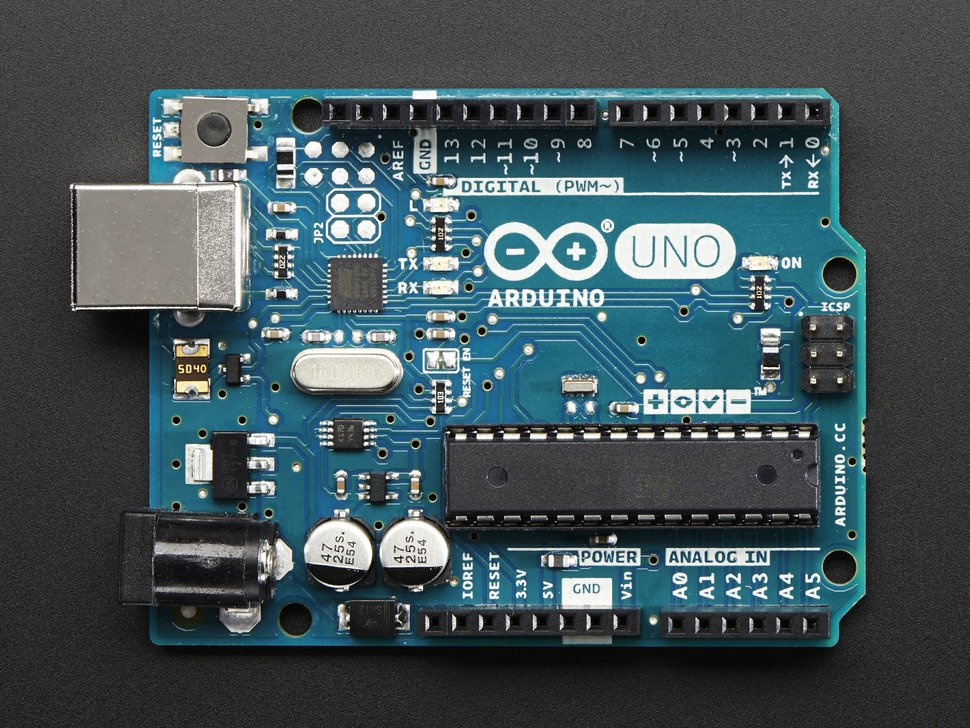
\includegraphics[width=1\textwidth]{figures/arduino2.JPG}}
	\caption{tampilan arduino}
	\label{arduino}
	\end{figure}
\subsection{Pengenalan Arduino}
 	Untuk memahami Arduino, pertama kita harus mengerti apa yang dimaksud dengan komputasi fisik. Komputasi fisik adalah untuk menciptakan suatu sistem atau perangkat fisik dengan menggunakan perangkat lunak dan perangkat keras yang interaktif sehingga dapat menerima rangsangan dari lingkungan dan merespon balik. Komputasi fisik adalah konsep untuk memahami hubungan manusia antara lingkungan yang sifatnya serupa dengan dunia digital. Dalam prakteknya konsep ini diterapkan dalam perancangan alat atau proyek yang menggunakan sensor dan mikrokontroler untuk menerjemahkan input analog ke dalam sistem perangkat lunak untuk mengendalikan pergerakan perangkat elektro-mekanis seperti lampu, motor dan sebagainya.
 	Arduino Uno merupakan board mikrokontroler yang memiliki basis ATM 328 atau datasheet. Arduino Uno memiliki 14 pin input dari output digital yang 6 pin input diantarnya dapat digunakan untuk outuot PWM dan 6 input lagi untuk analog, 16 MHz osilator kristal, jack power, tombol reset, ICSP header, dan koneksi USB. Untuk memaksimalkan kerja mikrokontroler agar dapat digunakan dengan maksimal sangat mudah caranya, hanya perlu menghubungkan Board Arduino Uno ke komputer menggunakan listrik dengan  AC yang ke arah  adaptor DC atau menggunakan kabel USB atau  juga bisa dengan menggunakan baterai untuk menjalankan Board Arduino Uno tersebut dan masih banyak cara lainnya.
  	Arduino Uno memiliki perbedaan dengan semua board yang telah diciptakan sebelumnya dalam hal koneksi USB to serial, yang dimaksud dengan koneksi USB to serial adalah menggunakan fitur Atmega 8U2 yang memiliki program sebagai konveter USB to serial yang berbeda dengan board yag telah diciptakan sebelumnya, pada board sebelumnya menggunakan chip FTDI driver USB to serial.
  	Uno berasal dari bahasa italia yang memiliki arti satu, hal ini digunakan untuk menandani peluncuran Arduino 1.0. Uno dan versi 1.0 yang akan menjadi versi referensi dari Arduino tersebut. Uno adalah seri terbaru dalam serangkaian board USB Arduino sekaligus menjadi model platform Arduino, dan menjadi perbandingan dengan versi Arduino sebelumnya.\cite{doukas2012building}
 %Definisi Arduino
 \section{Definisi Arduino}
  	Arduino adalah mikrokontroler singleboard opensource, berasal dari platform Wiring, yang telah disetting untuk memudahkan penggunaan elektronik di berbagai bidang. Perangkat kerasnya memiliki prosesor Atmel AVR dan perangkat lunaknya memiliki bahasa pemrograman tersendiri. Bahasa pemrograman yang digunakan arduino adalah bahasa pemrograman C atau C ++, hal ini dimaksudkan untuk memudahkan arduino untuk membaca codingan yang dibuat.
  	Arduino juga merupakan platform perangkat keras terbuka yang dapat digunakan untuk siapa saja yang ingin membuat prototip peralatan elektronik interaktif berdasarkan perangkat keras dan perangkat lunak yang fleksibel dan mudah digunakan. Mikrokontroler diprogram menggunakan bahasa pemrograman arduino yang memiliki kesamaan sintaksis dengan bahasa pemrograman C Karena sifatnya yang terbuka maka siapapun bisa mendownload skema hardware arduino dan membangunnya.
 	Arduino menggunakan keluarga mikrokontroler ATMega yang diluncurkan oleh Atmel, namun banyak perusahaan membuat buatan artifisial menggunakan mikrokontroler lainnya dan tetap kompatibel dengan arduino di tingkat perangkat keras. Untuk fleksibilitas, program ini dimuat melalui bootloader meski ada pilihan untuk bypass pada bootloader dan menggunakan downloader untuk memprogram mikrokontroler secara langsung melalui port ISP.\cite{jamieson2010arduino}

 %Sejarah Arduino
 \section{Sejarah Arduino}
 	Sejarah Arduino berawal dari sebuah tesis yang dibuat oleh seseorang bernama Hernando Baragan, di institute of Ivrea, Italia pada tahun 2005, kemudian dikembangkan oleh Massimo Banzi dan David Cuartielles dan diberi nama Arduin of Ivrea. Kemudian diganti nama menjadi Arduino yang dalam bahasa Italia berarti teman yang berani.
 	Tujuan awal dibuat Arduino adalah untuk membuat suatu perangkat mudah dan harganya murah, dari perangkat yang ada saat itu. Dan perangkat ini akan ditujukan kepada para siswa yang akan membuat perangkat desain dan interaksi.
 	Tim pengembangnya pada saat ini adalah Gianluca Martino, David Cuartielles, Tom Igoe, David Mellis, Massimo Banzi, dan Nicholas Zambetti. Mereka mengupayakan 4 hal dalam Arduino ini, yaitu:
 	1.	Harga yang terjangkau
 	2.	Dapat dijalankan di berbagai sistem operasi(OS). Seperti: Windows, Linux, Max, dan sebagainya.
 	3.	Sederhana, menggunakan bahasa pemograman yang mudah bisa dipelajari orang awam, bukan hanya untuk orang teknik saja.
 	4.	Open Source, baik hardware maupun software.

 %Jenis Jenis Arduino
 \section{Jenis-jenis Arduino}
a.	Terdapat beberapa jenis arduino jenis yang pertama adalah Arduino Fio, Arduino Fio memiliki bentuk yang lebih unik, terutama pada bagian socketnya. Meskipun mempunyai jumlah pin I/O digital dan juga input analognya sama dengan uno maupun leonardo,akan tetapi fio mempunyai socket XBeemembuat fio digunakanuntuk keperluan projek yang berhubungan dengan wireless. Selanjutnya Arduino Lilypad yaitu memiliki bentuk unik yaitu melingkar, lilypad dapat dipakai untuk membuat projek-projek yang unik tetapi juga dapat membuat suatu projek yang sangat keren.
 	Dengan 14 pinpin I/O digital, dan juga 6 pin input analognya.
 

b. Yang berikutnya merupakan arduino Nano seperti halnya dengan namanya "nano" yang memiliki arti ukuran  yang sangat kecil dan juga sangat sederhana ini, menyimpan banyak sekali fasilitas, dan juga sudah dilengkapi dengan FTDI untuk pemrograman yang melalui micro USB.Dengan dilengkapi 14 pin I/O digital, dan juga 8 pin input analog yang memiliki lebih banyak dari pada UNO. Dan ada juga yang menggunakan ATMEGA168 atau pun menggunakan ATMEGA328.
 
c. Untuk yang selanjutnya adalah jenis Arduino Mini dan juga jenis Arduino Micro.Arduino Mini memiliki fasilitas yang sama seperti yang dimiliki Arduino Nano yaitu menyimpan banyak sekali fasilitas, akan tetapi Arduino jenis ini tidak dilengkapi dengan Micro USB untuk pemrograman. Dan hanya memiliki ukuran 30mm x 18mm saja.
 Arduino Micro, Arduino jenis ini memiliki ukuran lebih panjang dari pada Arduino Nano dan juga Arduino Mini. Karena memang memiliki fasilitas yang lebih banyak yaitu memiliki 20 pin I/O digital dan juga 12 pin input analog.
 
 
d. Yang berikutnya adalah Arduino Ethernet dan Arduino Esplora. Arduino Ethernet, jenis arduino ini yang menyediakan beberapa cara dan beberapa protokol seperti HTTP, TCP, dan UDP yang memungkinkan terjadi program sketch yang menjadikan arduino sengai client atau server. Penjelasan client dan server merupakan software yang bentuk fisiknya dapat bermacam-macam seperti PC, mainframe, laptop dan microcontroller. Dan membuat arduino kamu dapat berhubungan langsung dengan LAN yang ada pada komputer. Untuk fasilitas pada pin I/O digital dan memiliki input analog yang sama dengan Uno. 
Ke dua yaitu Arduino Eksplora merupakan rekomendasi bagi kamu yang ingin membuat gadget seperti smartphone, karena sudah dilengkapi dengan LCD yang berfungsi untuk lebih mempercantik eksploranya.
 
e. Berikutnya merupakan Arduino Robot, arduini ini adalah paket yang lengkap dari arduino yang telah berbentuk robot. Dan juga telah dilengkapi dengan LCD, Speaker, Roda, Sensor Infrared dan juga semua yang kita butuhkan untuk pembuatan robot sudah ada di dalam arduino ini.

f. Arduino Uno
 Arduino ini adalah jenis arduino yang paling banyak digunakan saat ini. Khususnya untuk pemula yang baru belajar menggunakan arduino sangat disarankan untuk menggunakan Arduino Uno. Saat ini banyak sekali referensi yang membantu untuk mempelajari Arduino Uno. Versi Arduino yang terakhir adalah Arduino Uno R3 (Revisi 3), menggunakan ATMEGA328 sebagai Microcontrollernya, dan memiliki 14 pin I/O digital dan 6 pin input analog.Untuk pemograman cukup menggunakan koneksi USB type A to To type B. Sama seperti yang digunakan pada USB printer.

g. Arduino Due
 Berbeda dengan saudaranya, Arduino Due tidak menggunakan micro controller ATMEGA, melainkan dengan chip yang lebih tinggi ARM Cortex CPU. Memiliki 54 I/O pin digital dan 12 pin input analog.Untuk pemogramannya menggunakan Micro USB, terdapat pada beberapa handphone.

h. Arduino Mega Mirip dengan Arduino Uno, sama-sama menggunakan USB type A to B untuk pemogramannya. Tetapi Arduino Mega, menggunakan Chip yang lebih tinggi
  yaitu ATMEGA2560. Dan tentu saja untuk Pin I/O Digital dan pin input Analognya lebih banyak dari Uno.

i.Arduino Leonardo. 
 Bisa dibilang Leonardo adalah saudara kembar dari Uno. Dari mulai jumlah pin I/O digital dan pin input Analognya sama. Hanya pada Leonardo menggunakan Micro USB untuk pemogramannya.

%Manfaat dan fungsi Arduino
\section{Kegunaan atau fungsi Arduino}
 	    Arduino yang merupakan platfrom open source dapat digunakan oleh siapa saja yang ingin merancang prototipe peralaan elektronik interaktif dengan memanfaatkan fitur yang tersedia secara grafis dan fleksibel. Papan Arduino menggunakan jenis mokrokontroler ATMega yang diproduksi oleh Atmel sebagai chip utama. Walaupun demikian, saat ini sudah banyak perusahaan yang memproduksi dengan chip yang berbeda. Bahasa program yang digunakan adalah kompatibel dan diinput dengan bootloader atau dengan menggunakan downloader melalui port ISP. Karna arduino merupakan mikrokontroler open source, maka arduino bebas digunakan untuk membaca sensor serta mempu mengendalikan periperal motor, mesin dan lampu, ini memungkinkan setiap orang bebas mendowload.\cite{beug2012teaching}
%Konsep Arduino
\section{ Konsep Arduino}
\begin{figure}[ht]
	\centerline{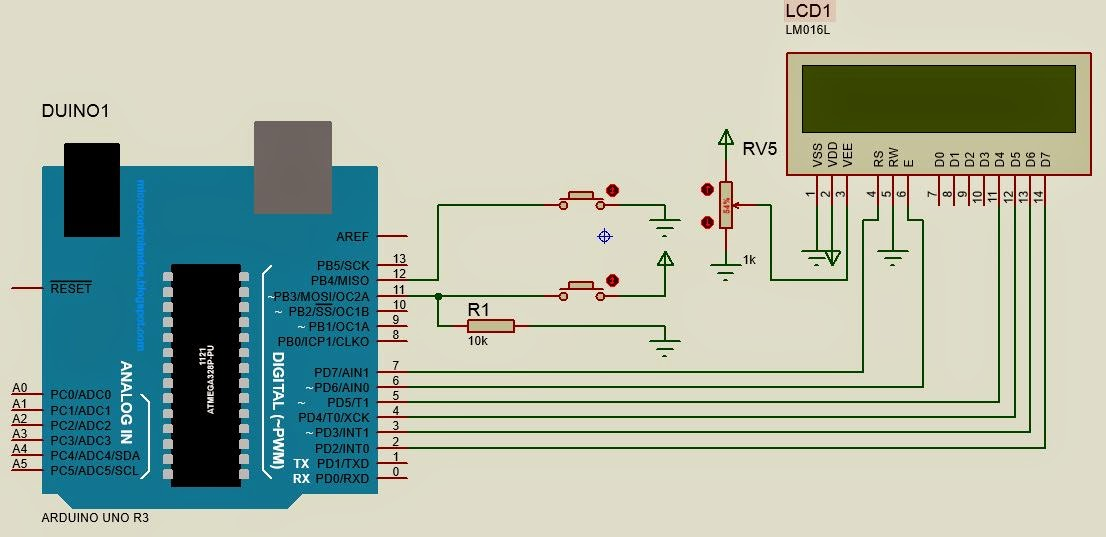
\includegraphics[width=1\textwidth]{figures/konsep.JPG}}
	\caption{tampilan konsep}
	\label{konsep}
	\end{figure}
 	Perangkat keras Arduino terdiri atas desain-desain hardware yang terbuka dengan prosesor Atmel AVR. Papan arduino dapat dibeli dengan pressembled, namun informasi dari desain perangkat keras juga tersedia untuk mereka yang ingin membangun ataupun memodifikasi. Adan beberapa pembuat pihak ketiga telah memproduksi Shield add-on board yang mampu memperluas kemampuan dasar dari arduino. Motor Control Shield memungkinkan untuk control motor DC dan pembentuk kode baca , perisai Xbee memungkinkan beberapa papan arduino untuk berkomunikasi secara nirkabel, dan Shield Velocity Accelorometer kritis menyatukan akselerometer 3 sumbu.  Pihak ketiga telah merilis beberapa variasi dari konsep arduino, ini merupakan papan bangunan perusahaan yang biasanya menggunakan spesifikasi lebih baik namun harga lebih rendah dengan menggunakan perangkat arduino.

 	Sumber Daya listrik. Papan pemrosesan Arduino mungkin didukung dari port USB selama pengembangan proyek.Namun, sangat disarankan agar catu daya eksternal dipekerjakan. Ini akan memungkinkan pengembangan proyek di luar kemampuan arus port USB yang terbatas. www.arduino.cc merekomendasikan catu daya dari 7-12 VDC dengan konektor positif pusat 2,1 mm. hal ini bertujuan agar daya yang terkonek pada arduino lebih stabil
 
 	Catu daya jenis ini sudah tersedia dari sejumlah perusahaan pemasok komponen elektronik.Misalnya, catu daya jameco 133891 adalah model 9 VDC yang diberi nilai 300 mA dan dilengkapi dengan konektor positif pusat 2,1 mm. Tersedia dengan harga di bawah 10 US dollar, catu daya ini memiliki harga yang tidak terlalu mahal sehingga sebagian besar orang menggunakan produk tersebut.

 	Perangkat lunak ini terdiri dari bahasa pemrograman standar dan firmware yang berjalan di papan tulis. Perangkat keras Arduino diprogram menggunakan bahasa yang disederhanakan C ++, dalam IDE berbasis pengolahan. Perangkat lunak ini kemudian disusun dan dimuat di kapal. Papan Arduino juga kompatibel dengan Flash, Processing, MaxMSP, dan MATLAB, dan beberapa baris kode seringkali cukup untuk memungkinkan perilaku yang cukup kuat
 
 	Struktur pemrograman dasar Arduino terdiri dari setidaknya dua bagian. Ini adalah komponen setup dan loop. Pada set-up, yang berjalan di awal dan hanya sekali untuk mengatur mode pin atau komunikasi serial, variabel-variabel tersebut dideklarasikan. Bagian kedua berjalan dalam satu lingkaran yang memungkinkan skrip untuk berubah, merespons, dan mengendalikan dewan Arduino. Setelah mendeklarasikan variabel, mengendalikan Arduino melibatkan struktur kontrol klasik (IF, IF ... ELSE, FOR, dll.), Operator aritmatika (+, -, /, *, dll.), Dan operator perbandingan (>, <, dan lain-lain) atau boolean (DAN, ATAU, dll.). 
 	
 	Ada juga seperangkat perintah untuk membaca dan menulis analog dan digital seperti digitalwrite () atau digitalread (). Selanjutnya, perintah lainnya dapat mengatur penundaan temporal dalam milidetik, melakukan operasi matematis dan trigonometri dasar (min / max, nilai absolut, akar kuadrat, sinus, kosinus, dll.), Atau menghasilkan bilangan acak. Untuk informasi lebih lanjut, lihat tutorial web atau ke dokumentasi resmi.

 	Sebagai contoh penggunaan praktis, anggaplah bahwa peserta eksperimen harus menjangkau dan memahami suatu objek, dan seorang peneliti ingin memicu mesin lain (yaitu mesin Stimulasi Magnetik Transkranial) 100 ms setelah kontak objek. Solusi yang khas adalah sensor sentuh yang berkomunikasi, melalui port paralel, dengan program perangkat lunak pada komputer (yaitu, E-Prime atau Presentation)

 	Papan Arduino juga memiliki tugas sebagai I / O pada tingkat rendah yang diperlukan untuk mengatur yang tidak konvensional  pada perangkat keras tambahan, memerlukan beberapa solusi kreatif yang dapat membantu, dan untuk keterampilan pemograman. Perhitungkan, contohnya, daftar singkat pada proyek terbuka yang mungkin akan sangat berguna di dalam laboratorium psikologis dan neurofisiologis. Sensor sentuhan yang sangat mudah untuk dibangun dan murah harganya telah dirancang untuk digunakan dalam penelitian perilaku yang melibatkan pengukuran waktu reaksi atau disingkat RT peserta yang telah mencapai dan menyentuh benda tersebut. Proyek lain menunjukkan bagaimana cara membangun fotodioda yang dapat digunakan, misalnya, untuk mendeteksi presentasi stimuli pada layar.Dan akhirnya, satu proyek lain ini menunjukkan bagaimana cara untuk mengenalkan kemampuan debouncing ke masukan apa pun, yang sangat berguna mengingat fakta yang diketahui bahwa sebagian besar bahkan hampir semuanya bantalan tombol menawarkan sinyal yang tergolong berisik, dan yang dimaksud debouncing adalah langkah yang diperlukan untuk memilih RT yang benar.\cite{fatoni2017perancangan}